\section{Screens}
\label{sec:screens}

This chapter describes all the available screens.

\subsection{Math test}
\label{sec:screens-math-test}

The math test screen is the main stress-inducing factor of the stress test.
The stress is induced by mathematic questions. 
For each question, the user has only a limited time to answer the question. 
If the time is over or the user has given the wrong answer, a negative feedback message is displayed. 
If the user has answered the math question correctly a positive feedback message is displayed. 
The feedback message is visible for a short amount of time. 
After this short pause, a new question is displayed.
Math questions are taken out of a pool of 40 arithmetic expressions. 
Before every math test, the array of questions is mixed randomly.

\begin{figure}[htb]
  \centering
  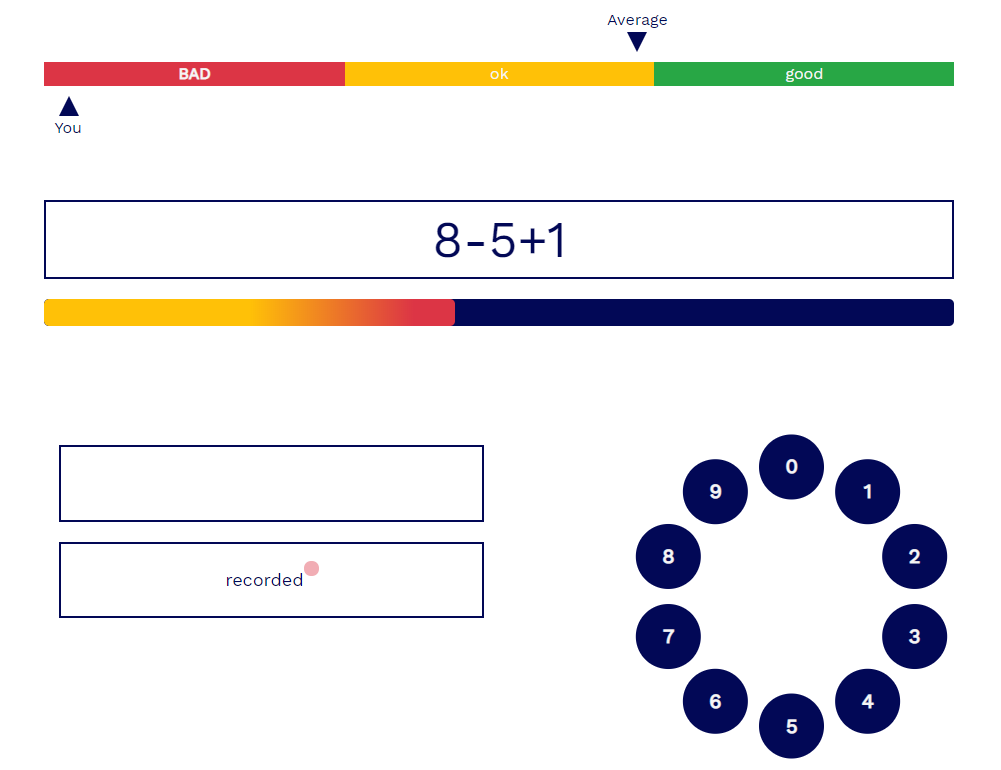
\includegraphics[width=\textwidth]{figures/Math-test.png}
  \caption{Screenshot of the math test screen}
  \label{fig:screenshot-math-test-screen}
\end{figure}

Figure \ref{fig:screenshot-math-test-screen} shows a screenshot of the math test screen.
At the top, the level bar is displayed, which shows two indicators "You" and "Average".
The "You" indicator shows the real performance of the participants.
The "Average" indicator is faked.
It is just increasing if the participant has given a correct answer and is decreasing if the participant has given an incorrect answer.
Below the math questions, a progress bar is displayed.
It shows the remaining time for the participant to answer the current question.
The user must give their answers with the dial pad at the right bottom of the screen.
The feedback is given inside the blue box on the left of the screen.

\subsubsection*{Settings of the math screen}

\paragraph{Enable sound}
If enabled, feedback will be given also via sound. 
To induce more stress an annoying background sound is played while the user has time to answer the math question.
Note: users can turn their volume down or mute their speakers, so do not rely on the sound to be heard.

\paragraph{Activate Control}
This option enables the control mode.
During control mode, the level bar and progress bar are hidden.
Also, the annoying background sound will not be played.

\paragraph{Total test time}
The total duration in seconds of the math test.

\paragraph{Answer timeout}
The duration in seconds for answering one math question.

\paragraph{Time between questions}
The duration in seconds of the short pause after the feedback of the current question has been given to the user.

\paragraph{Difficulty}
The initial difficulty of the math questions.
The table \ref{tab:math-test-difficulty} lists all possible difficulty levels.
The difficulty level will be increased by one level if the participant has answered three questions correctly in a row.
The level is decreased by one level if the participant has answered three questions incorrectly in a row.

\begin{table}[ht]
  \begin{tabularx}{\textwidth}{l|l|l|l}
    level & number of operands & possible operators & example \\
    \hline
    $0$ & $2$ & $+$, $-$ & $7-2$ \\
    $1$ & $3$ & $+$, $-$ & $2-5+6$ \\
    $2$ & $3$ & $+$, $-$, $*$ & $3*5-9$ \\
    $3$ & $4$ & $+$, $-$, $*$ & $2*4-2*3$ \\
    $4$ & $4$ & $+$, $-$, $*$, $/$ & $3*6/2-2$ \\
  \end{tabularx}
  \caption{Difficulty levels for the math test}
  \label{tab:math-test-difficulty}
\end{table}

\subsection{Message}
\label{sec:screens-message}
The message screen shows a simple message to the user.
The user can go to the next screen by clicking a button on the screen.
The title, the message and the button text of this screen can be adjusted.

\subsection{Wait Screen}
\label{sec:screens-wait-screen}
The wait screen shows a simple message to the user, like the \nameref{sec:screens-message} screen.
But the user must wait a specific time until the next screen is displayed.
The user cannot manually go to the next screen.
The title, the message, and the waiting duration in seconds of this screen can be adjusted.

\subsection{Chatbot}
\label{sec:screens-chatbot}
This screen provides a very basic chatbot functionality.
Stress test creators can define the chat messages the chatbot will show to the participant.
After the chatbot has sent a message to the participant, he must send an answer to the chatbot.
After the last message from the chatbot, a "Click to continue" button will be displayed, which will take the participant to the next screen.
The answer a participant has given will be added to the statistics of this test execution.

\subsection{Start}
\label{sec:screens-start}
This screen can be used as the first screen.
It displays the Stress+ logo and can show a custom message.

\subsection{End}
\label{sec:screens-end}
This screen can be used as the last screen.
It displays the Stress+ logo and can show a custom message.

Note: The end screen has no mechanism to go to the next screen. 
Therefore, it should not be placed in the middle of the pipeline.
If the end screen is not present a blank page will be shown as the last screen.

\subsection{Survey}
\label{sec:screens-survey}
The survey screen can display other websites inside the stress test. 
This can be useful to display for example a Google Form inside a stress test.
A button will always be displayed at the top of the screen to navigate to the next screen.
